\documentclass[tikz,border=4pt]{standalone}
% Shared setup for the foundation-model diagrams, in the AFRICAST palette
\usepackage{fontspec}
\usepackage[sfdefault]{FiraSans}
\usepackage{amsmath}
\usepackage{unicode-math}
\setmathfont{Fira Math}
\usetikzlibrary{arrows.meta}
\definecolor{ink}{HTML}{1F2A36}
\definecolor{MonashBlue}{HTML}{3B75AC}
\definecolor{Orange}{HTML}{B5570F}
\color{ink}
\tikzset{every picture/.style={draw=ink,>=stealth}}
\hyphenpenalty=10000
\exhyphenpenalty=10000

\begin{document}
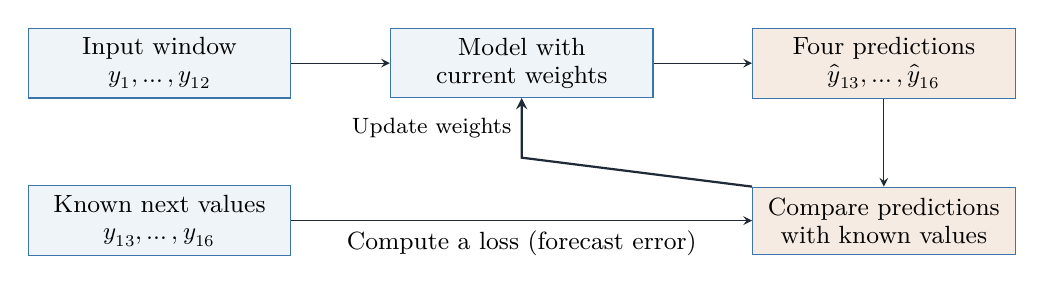
\begin{tikzpicture}[>=stealth,every node/.style={font=\fontsize{9}{10}\selectfont,align=center},
box/.style={draw=MonashBlue,fill=MonashBlue!8,text width=3.1cm,minimum height=.85cm}]
\node[box] (x) at (0,0) {Input window\\$y_1,\ldots,y_{12}$};
\node[box] (m) at (4.6,0) {Model with\\current weights};
\node[box,fill=Orange!12] (p) at (9.2,0) {Four predictions\\$\hat y_{13},\ldots,\hat y_{16}$};
\node[box] (y) at (0,-2) {Known next values\\$y_{13},\ldots,y_{16}$};
\node[box,fill=Orange!12] (loss) at (9.2,-2) {Compare predictions\\with known values};
\draw[->] (x)--(m);\draw[->] (m)--(p);\draw[->] (p)--(loss);
\draw[->] (y)--node[below]{Compute a loss (forecast error)}(loss);
\draw[->,thick] (loss.north west)--(4.6,-1.2)--node[left,font=\fontsize{8}{9}\selectfont]{Update weights}(m.south);
\end{tikzpicture}
\end{document}
